\documentclass[pdftex,12pt,a4paper]{report}

\usepackage[pdftex]{graphicx}
\usepackage[ansinew]{inputenc}
\usepackage{geometry}
\usepackage{bbold}
\usepackage{program}
\usepackage[toc,page]{appendix}
\usepackage{subcaption}
\geometry{a4paper,left=2.5cm,right=2.5cm, top=2.5cm, bottom=3cm}
\newcommand{\HRule}{\rule{\linewidth}{0.5mm}}

% definition for ToC

\usepackage{lipsum}% http://ctan.org/pkg/lipsum
\usepackage{titletoc}% http://ctan.org/pkg/titletoc
\titlecontents*{chapter}% <section-type>
  [0pt]% <left>
  {}% <above-code>
  {\bfseries\chaptername\ \thecontentslabel\quad}% <numbered-entry-format>
  {}% <numberless-entry-format>
  {\bfseries\hfill\contentspage}% <filler-page-format>

\begin{document}
\begin{titlepage}


%%LR
\sffamily

\begin{center}


% Oberer Teil der Titelseite:

\includegraphics[width=0.3\textwidth]{logo2.jpg}
\hfill

\includegraphics[width=0.4\textwidth]{logo1.jpg}  
\\[5cm]

{\Large Department of Mathematics}\\[0.5cm]
{\Large Chair of Mathematical Modeling of Biological Systems}\\[0.5cm]
{Technische Universit\"at M\"unchen}\\[2cm]
{\Large Master's Thesis in Bioinformatics}\\[1.5cm]

% Title
\HRule \\[0.4cm]
{ \huge \bfseries Single-cell analysis of cancer drug response using computer vision and learning algorithms on time-lapse microtrench data}\\[0.4cm]

\HRule \\[1.5cm]

{\Large Pandu Raharja}\\[2.5cm]

\vfill
\end{center}
\end{titlepage}
\pagestyle{empty}

%%LR comprehensive title
\begin{titlepage}
{\sffamily


\begin{center}

\includegraphics[width=0.3\textwidth]{logo2.jpg}
\hfill

\includegraphics[width=0.4\textwidth]{logo1.jpg}  
\\[1.5cm]  

{\Large Department of Mathematics}\\[0.5cm]
{\Large Chair of Mathematical Modeling of Biological Systems}\\[0.5cm]
{Technische Universit\"at M\"unchen}\\[1cm]

{\Large Master's Thesis in Bioinformatics}\\[2cm]
{\textbf{\Large Single-cell analysis of cancer drug response using computer vision and learning algorithms on time-lapse microtrench data}}\\[2cm]
{\textbf{\Large Wirkungsanalyse von Krebsmedikamenten in Einzeller Aufl\"osung durch die Anwendung von Computer-Vision- und Machine-Learning-Algorithmen auf Microtrench- Videoaufnahme}}\\[4cm]

\end{center}
\begin{center}\Large
  \begin{tabular}{ll}
    Author:& Pandu Raharja\\
    Supervisor: &  Prof. Dr. Fabian Theis, Dr. Carsten Marr\\
    Advisor:        &  Prof. Dr. Fabian Theis\\
    & Prof. Dr. Dmitrij Frishman\\
    Submitted:     &  15.10.2017
  \end{tabular}
\end{center}

}% end title page

\end{titlepage}


%%%%%%%%%%%%%%%%%%%%%%%%%%%%%%%%%
% thesis content starts here
%%%%%%%%%%%%%%%%%%%%%%%%%%%%%%%%%

\newpage


\begin{abstract}
Quantitative measurement of cancer drug response is esential to objectively gauge the efficacy of cancer drugs. So far, there has been no method to track and  quantitatively measure single-cell response of of cancer drug treatment. A novel pipeline is presented in this thesis. First, a quasi-high-throughput method to track cells and quantitatively analyze single-cell response to drugs. We investigate the response of model cancer cell lineagues, MOLM and Jurkat, to known anti-cancer drugs Vincristine and Doxorubicine. While the method enabled relatively easy and quasi-high-throughput analysis of cancer treatment \textit{in vitro}, our pipeline could also be adapted in varios contexts involving single-cell analysis with reasonable amount of modifications necessary.
\end{abstract}

\newpage

\tableofcontents

\newpage

\chapter{Introduction}

In almost every part of the world, cancer is either the most or second most deadly family of diseases. 

Cancer is among the most deadly family of diseases ever known to human being. In 2016, TODO: put study

\lipsum[1]

\begin{verbatim}
I.
- readable to people without background in the fields
- non technical at all
II.
- what have the researches done
-- biologics
-- technicals
III.
thesis overview
4~8 pages
\end{verbatim}

\section{Test}

\lipsum[2]

\chapter{Data and Methods}

This chapter will consider two aspects of the project: the experiment setting and the data analyis pipeline. In the first half of the chapter, the cell environment is brouht forth. The highlight of this experiment, the microslit setup for cell containment, is elucidated in this part. Also, the drugs that are tested on the cell cultures are exhibited. After that, the cell lines used in this experiment are explained with context of the aim of the experiment. Later on, the experiment treatment and the hypothesis is presented.

The second part deals mostly with the quantitative methods used to process data into meaninful observations. The part is opened with definitions used in the methods section. Afterwards, each method developed/used in the pipeline is brought forward. For each method, the rationale explaining the reason of using the method is also accompanied in the subsection.

\section{Experimental Setting and Data}

\lipsum[1]

\section{Definitions}

Mathematical definitions used in the thesis

\section{Methods}

\lipsum[1]

\subsection{Laplacian of Gaussian (LoG) Cell Recognition}

\lipsum[1]

\subsection{Image Encoding}

Consider whether image encoding shoud contain Lenna's picture instead.

\subsection{Shift Correction}

Consider following picture:

\begin{figure}[h]
\centering
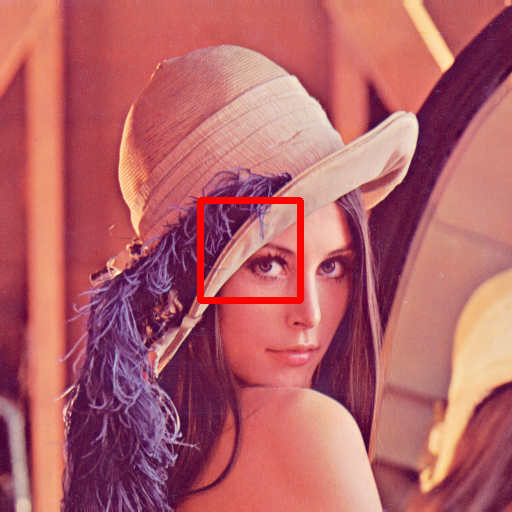
\includegraphics[width=0.5\textwidth]{lenna_marked}
\label{fig:lenna}
\caption{Lenna}

\end{figure}

There are numerous encodings that could be used to internally represent this picture. Many such encodings derived from the so-called Red-Green-Blue (RGB) encodings. RGB encoding represents the pixel as a combination of red, green and blue color. This encoding is able to represent various spectra of human visible color and useful enough for most use cases (citation). To give representation on how the encoding works, the RGB encoding of some part of Figure \ref{fig:lenna} is shown in Figure \ref{fig:lennas}. For an image of size $m \times n$ pixels, the RGB encoding is thus a 3-dimensional matrix of dimension $m \times n \times 3$. For time-lapsed images accordingly, the RGB encoding of a video of length $T$ is a 5-dimensional matrix of shape $T \times m \times n \times 3$. TODO: put graphical explanation of data here.

%An expansion of such encoding, the RGBH encoding, expands the representation by adding the brightness of the pixel -- known as 'hue'.

\begin{figure}[h]
\begin{subfigure}{.5\textwidth}
  \centering
  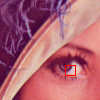
\includegraphics[width=.8\linewidth]{lenna_marked_small}
  \caption{1a}
  \label{fig:lennas1}
\end{subfigure}%
\begin{subfigure}{.5\textwidth}
  \centering
  
\includegraphics[width=.8\linewidth]{lenna_small}
  \caption{1b}
  \label{fig:lennas2}
\end{subfigure}
\centering
\begin{subfigure}{.5\textwidth}
  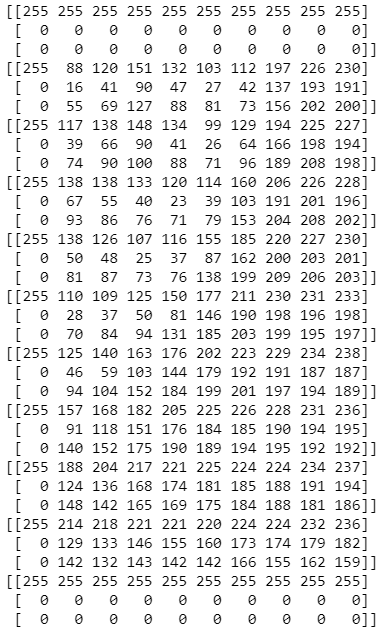
\includegraphics[width=.8\linewidth]{lenna_rbg}
  \caption{1b}
  \label{fig:lennas3}
\end{subfigure}
\caption{Figure \ref{fig:lennas1} shows the content of red marked region in Figure \ref{fig:lena}. Figure\ref{fig:lennas2} shows the zoomed part around Lena's right eye and matrix represented in Figure \ref{fig:lennas3} shows the RGB representation of the eye.}
\label{fig:lennas}
\end{figure}


Now, consider a case in which images are shifted in a time-lapsed movie. TODO: explain mechanism. No rotation of camera is assumed, hence there are only two degree of freedoms (vertical and horizontal). Thus, a shift can be defined as a vector movement $\vec{v}$ of all points $x_{i,j} \in M_{t_i}$ in the time-lapse from time $t_i$ to $t_{i+1}$. Given two degrees of freedom and discreteness of the problem due to pixel representation, the task is reduced to finding difference in x- and y-axis ($\delta_x$ and $\delta_y$), so that the difference of transformed pixels at $t_i$ and $t_{i+1}$ are minimized, i.e.:

$$
argmin_{\delta_x, \delta_y} \{d(M_{t_i}, M_{t_{i+1}}^{\delta_x, \delta_y} + (\delta_x, \delta_y)^T)\}
$$

Where $M_{t_{i+1}}^{\delta_x, \delta_y}$ is the entries of matrix $M_{t_{i+1}}$ after applying the shift $\vec{v} := (\delta_x, \delta_y)^T$, i.e.

$$M_{t_{i+1}, \, x, \, y}^{\delta_x, \delta_y} = M_{t_{i+1}, \, x - \delta_x, \, y - \delta_y}$$

For the distance function $d$, the in all channels absolute difference function is used, which is defined as:

$$
d(M_i, M_j) = \sum_{c \, \in \, \{R, B, G\}} \sum_{x} \sum_{y} \vert M_{i, c, x, y} - M_{j, c, x, y} \vert
$$


Since some pixels are lost from the field of view during a shift, only a subset of subsequent pictures is used to determine the shift, preferably those around the center point. This will allow the largest search space possible, since the distance to all four margins of the picture is maximized at the center point. The search for the optimal $(\delta_x, \delta_y)$ pair is implemented as a grid search along the x- and y-axis. An example of the search grid is shown in Figure \ref{fig:searchgrid}.\\

\begin{figure}[h]
\centering
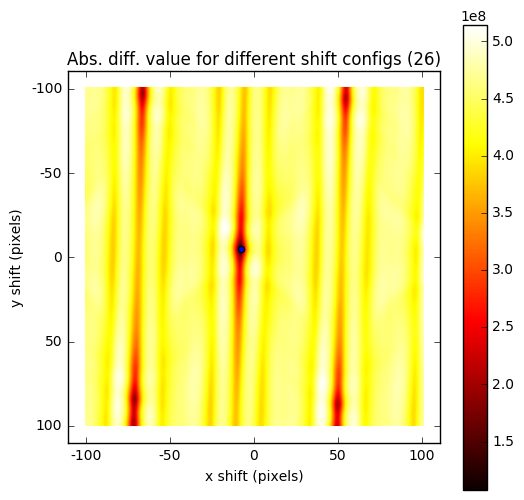
\includegraphics[width=0.5\textwidth]{search_grid}
\caption{Search grid shift for Position 26. The search was conducted for shift between the last time point before and the first time point after the drugs treatment. The minimum is marked with thick black dot, which is returned after every grid-search call as inferred shift. In the position, the shift was inferred to be 8 pixels upwards and 5 pixels leftwards. Notice the repeating pattern of relatively favorable configurations after approximately 50 horizontal and 100 vertical pixels caused by lattice nature of the slits.}
\label{fig:searchgrid}
\end{figure}

%% TODO: RESTRUCTURE THE CHAPTER

Since the time-lapsed data consists mainly of grayscale image, the RGB encoding could be the directly transformed to grayscale encoding. Using the transformed method also speeds up the calculation process since the distance function only computes the difference of grayscale channel's values:

$$
d(M, N) =  \sum_{x} \sum_{y} \vert M_{c, x, y}^{gray} - N_{x, y}^{gray}\vert
$$

Due to lost pixels around the margin of before and after pictures, only the overlapping part of both slides are included after the correction. Thus, for an inferred shift of $(\delta_x, \delta_y)$, the new dimension of the pictures is then $(m - \delta_x) \times (n - \delta_y)$. This change would then propagation to the other time-lapse images to maintain consistency of the images.\\

Ideally, the shift correction should be done for each position to reduce the track dropout rate caused by image shifts. This is however computationally very expensive and, as seen in Figure \ref{fig:pixdiff}, not really necessary since the biggest shift indeed only happens right before and after the treatment, as it was expected during the experiment setting. As seen in Chapter XX (TODO: quote), the tracking allows certain amount of tolerance. In this regard, the other frame shifts are way within the tolerance of our tracking algorithm. As shown in Figure YY (TODO: add droput rate), the dropouts caused by frame shifts in the other time points are basically noisy dropout caused by random noise in time-lapse movie being tracked as cells (TODO: add reference about this phenomena).

The algorithm for shift inference could be seen in Appendix \ref{appendix:graph}.

\begin{figure}[h]
\centering
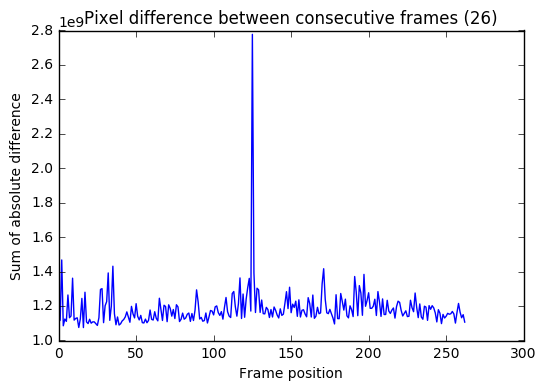
\includegraphics[width=0.8\textwidth]{pixdiff}
\caption{Pixel difference between consecutive frames at Position 26. In most cases, the pixel difference between the frames is mainly caused by moving cells. The diference during the treatment, on the other hand, is caused by physical shift of the frame. While moving cells mostly caused minimum noise-like pixel difference, the physical shift of field of view distorts the physical alignment and evokes immense pixel difference.}
\label{fig:pixdiff}
\end{figure}

\subsection{Cell death signals}

Measuring cell death is a crucial part of the experiment, as the reliable determination of it is the basis of most analysis in this thesis. There are several way to measure cell deaths with varying complexity and accuracy. Each method contains certain assumptions of cell death.\\

For example, determining cell death by cell movement assumes death of a cell if no movement beyond random flux is observed in certain amount of time. This obviously has certain drawbacks, such as when the observation is done in non-static environment. Moreover, defining the limit of the random flux, above which a given cell is assumed to actively move, is not a trivial task. Some kind of gold standard for a given cell line and environment has to be established manualy, which is very time consuming. This fact is again made even more complicated by the fact that many cells show different movement pattern upon introduction of treatment (TODO citation). It is well known that some cells tend to move faster or slower under stress (TODO citation), the situation many cancerous cells in our experiment will experience upon addition of cancer drugs treatment (TODO citation).\\

The second method is using cell size. During apopotosis, the cells would shrink. Given It is known that cell size 




In this experiment, two cell signals are used as indicator of cell death.


\chapter{Results}

\lipsum[1]

\begin{verbatim}
I. Pipeline

II. Quantitative Analysis
\end{verbatim}

\chapter{Summary and Outlook}

\lipsum[1]

\begin{verbatim}
I. Summary (and discussion?)
Connect Results with Background

II. Outlook
Improvemnt capability
\end{verbatim}

\lipsum[1]

\begin{appendices}

\chapter{Algorithms}\label{appendix:graph}

\lipsum[1]

\section*{Shift Inference} 

\begin{verbatim}
def infer_shift(last_slide, first_slide, search_space=(200, 200)):
    
  if (search_space[0] % 2 != 0) or (search_space[1] % 2 != 0):
    print("Search spaces have to be even!")
    return None
  else:
    
    ## calculate absolute difference for various shifts
    x1 = search_space[0]
    x2 = search_space[0]
    y1 = search_space[1]
    y2 = search_space[1]
    mid = f1.shape[0] // 2, f1.shape[1] // 2
        
    ## results storage        
    absdiffs = np.zeros((search_space[0] + 1, search_space[1] + 1))

    ## last slide before treatment
    f1sub = f1[(mid[0] - x1):(mid[0] + x2), (mid[1] - y1):(mid[1] + y2)]
    
    ## search space 
    xdiff1 = -int(search_space[0] / 2)
    xdiff2 = int(search_space[0] / 2) + 1
    ydiff1 = -int(search_space[1] / 2)
    ydiff2 = int(search_space[1] / 2) + 1
    
    for xdiff in range(xdiff1, xdiff2):
      for ydiff in range(ydiff1, ydiff2):
      
        ## calculate absolute difference for shift
        f2sub = f2[(mid[0] - x1 + xdiff):(mid[0] + x2 + xdiff), 
                   (mid[1] - y1 + ydiff):(mid[1] + y2 + ydiff)]
        x = xdiff + int(search_space[0] / 2)
        y = ydiff + int(search_space[1] / 2)
        absdiff_xy = np.sum(cv2.absdiff(f1sub, f2sub).ravel())
        absdiffs[x][y] = absdiff_xy
        
        
    ## calculate shift based on calibration data
    x = np.argmin(absdiffs) // absdiffs.shape[0]
    y = np.argmin(absdiffs) % absdiffs.shape[0]
    
    """
    True shift is the opposite of coordinate encoded
    in absdiff
    
    Let X2 the second picture and X1 the first picture.
    If the sub-picture of first slide of X2 centered
    at (c1 + s1, c2 + s2) fits the most with the sub-picture
    of the last slide of X1 centered at (c1, c2)
    then the pictures shift by (-s1, -s2) upon treatment
    """
    diff = -(x - search_space[0] / 2), -(y - search_space[1] / 2)

    return diff
\end{verbatim}

\end{appendices}

\end{document}